\chapter{The Score as Posterior Expectation: Belief Propagation and the
Gaussian Closure}\label{ch:bp}

Chapter~\ref{ch:gaussian} computed the joint score by inverting a
$K \times K$ matrix; Tweedie's identity (Section~\ref{sec:tweedie}) says the
same object is a posterior expectation. This chapter takes the Bayesian
route seriously and rebuilds the score by \emph{message passing}: local
computations on the factor graph of the posterior. The questions answered
are RQ2 and RQ3. First we show that belief propagation computes the score
of the Gaussian chain \emph{exactly}, in $O(K)$, and that the algorithm is
--- update by update --- the classical Kalman filter and smoother. The
closure of Gaussian messages is pure algebra, not a central-limit argument:
this resolves, in the affirmative and with a precise mechanism, the first
conjecture of the supervision discussion that shaped this chapter. Second,
we analyse the per-node Gaussian closure (AMP, the TAP equations of
statistical physics) and prove the second half of that discussion --- ``a
CLT on two data points is usually not right'' --- as a theorem: on the
chain, AMP still returns the exact score, but its variance closure
develops an exact breakdown time $t_c(\alpha)$ with critical coupling
$\alpha_c = \sqrt{2} - 1$. Third, we quantify the Gaussian closure on
genuinely non-Gaussian chains, using deterministic grid quadrature as exact
reference, and extract the locality lessons for learned score
architectures.

\section{The computational problem}\label{sec:bp-problem}

Fix the setting of Chapters~\ref{ch:gaussian}--\ref{ch:laplace}: a Markov
chain prior $P_0(a) = p_0(a_0) \prod_k M(a_{k+1} | a_k)$, per-frame OU
evidence, and the posterior
\begin{equation}
  p(a \,|\, x) \;\propto\;
  \underbrace{\psi_{\mathrm{pr}}(a_0)
  \prod_{k=0}^{K-2} \psi^{(k)}_{\mathrm{tr}}(a_k, a_{k+1})}_{\text{chain prior}}
  \;
  \underbrace{\prod_{k=0}^{K-1} \psi^{(k)}_{\mathrm{ob}}(a_k)}_{\text{evidence}},
  \qquad
  \psi^{(k)}_{\mathrm{ob}}(a_k) = \Nd\big(x_k;\, e^{-t}a_k,\, \Deltat\big).
  \label{eq:bp-posterior}
\end{equation}
By Tweedie, the $k$-th score component needs the posterior mean
$\E[a_k | x]$ --- a marginal of \eqref{eq:bp-posterior}. Computing $K$
marginals naively costs $O(K^2)$ one-dimensional eliminations ($O(K^3)$ by
matrix inversion in the Gaussian case); message passing computes \emph{all}
of them in one forward and one backward sweep, $O(K)$ total. The gain is
not merely computational: the message-passing form exposes \emph{which}
information reaches frame $k$ from where --- exactly the structural
question RQ4 asks.

\subsection{The factor graph is a tree}

The factor graph of \eqref{eq:bp-posterior} has $K$ variable nodes, $2K$
factor nodes ($1$ prior, $K{-}1$ transitions, $K$ observations --- the data
$x_k$ are constants clamped inside their factors, not nodes), and
$3K - 1$ edges: each transition factor has degree $2$, prior and
observations degree $1$. A connected graph with (nodes${}-1$) edges is a
tree. Pictorially it is a \emph{caterpillar}: a spine of variables and
transition factors, one evidence leaf per vertebra --- in the words of the
supervision discussion, ``very tree-like: a straight line with things on
the side''. Every interior variable has degree three; every message update
combines a \emph{small, fixed} number of inputs. Two consequences, one per
half of this chapter: BP on a tree is exact
\citep{pearl1988probabilistic, mezard2009information}; and this graph is
the diametrical opposite of the dense, high-degree graphs for which the AMP
closure was invented --- which is where the BP/AMP contrast will come from.

\subsection{Sum--product, and the continuous-message obstruction}

On a generic factor graph, sum--product BP passes messages along every edge
\citep{kschischang2001factor, mezard2009information}:
\begin{equation}
  \nu_{i \to a}(a_i) \propto
    \prod_{b \in \partial i \setminus a} \hat\nu_{b \to i}(a_i),
  \qquad
  \hat\nu_{a \to i}(a_i) \propto
    \int \psi_a(a_{\partial a})
    \prod_{j \in \partial a \setminus i} \nu_{j \to a}(a_j)\;
    \dd a_{\partial a \setminus i},
  \label{eq:bp-rules}
\end{equation}
with the belief at node $i$ proportional to
$\prod_{a \in \partial i} \hat\nu_{a \to i}(a_i)$. On a tree these
equations have a unique solution, reached in one inward and one outward
pass, and the beliefs are the exact marginals
\citep[Theorem~14.1]{mezard2009information}.

For \emph{discrete} variables each message is a finite probability vector
and \eqref{eq:bp-rules} is straightforward arithmetic. For
\emph{continuous} variables each message is a probability \emph{density} ---
an infinite-dimensional object --- and the update integrals must be carried
out in function space. This is the obstruction, identified sharply in
supervision, that makes ``BP on continuous chains'' a research question
rather than a textbook exercise: tree-exactness of the \emph{algorithm} is
untouched, but the \emph{representation} of messages becomes the whole
problem. There are exactly three ways out: (i) discrete data (retreat to
finite alphabets); (ii) a conjugate family closed under the updates ---
the Gaussian route, exact for our Gaussian chain, as we prove next;
(iii) numerical function representation --- the grid route, which we use
in Section~\ref{sec:bp-nongaussian} as exact reference for non-Gaussian
chains.

\section{Belief propagation on the chain}\label{sec:bp-chain}

On the chain, \eqref{eq:bp-rules} collapses into one forward and one
backward sweep. The bookkeeping deserves unusual care --- an earlier
version of this project's notes fell into a trap here, caught only by the
numerical audit.

\begin{proposition}[Convention A]\label{prop:bp-convA}
Define messages
\begin{align}
  \mu_{\to 0}(a_0) &:= \psi_{\mathrm{pr}}(a_0),
  &
  \mu_{\to k+1}(a_{k+1}) &:= \int
    \psi^{(k)}_{\mathrm{tr}}(a_k, a_{k+1})\,
    \psi^{(k)}_{\mathrm{ob}}(a_k)\,
    \mu_{\to k}(a_k)\; \dd a_k ,
  \label{eq:bp-fwd}\\
  \mu_{\leftarrow K-1}(a_{K-1}) &:= 1,
  &
  \mu_{\leftarrow k-1}(a_{k-1}) &:= \int
    \psi^{(k-1)}_{\mathrm{tr}}(a_{k-1}, a_k)\,
    \psi^{(k)}_{\mathrm{ob}}(a_k)\,
    \mu_{\leftarrow k}(a_k)\; \dd a_k .
  \label{eq:bp-bwd}
\end{align}
Then for every $k$,
\begin{equation}
  p(a_k \,|\, x) \;\propto\;
  \mu_{\to k}(a_k)\;
  \psi^{(k)}_{\mathrm{ob}}(a_k)\;
  \mu_{\leftarrow k}(a_k) :
  \label{eq:bp-combine}
\end{equation}
the forward message into $a_k$ carries the evidence $x_0, \dots, x_{k-1}$
only, the backward message carries $x_{k+1}, \dots, x_{K-1}$ only, and the
local evidence enters once, at combination time.
\end{proposition}

The proof is direct marginalisation: integrating \eqref{eq:bp-posterior}
over all $a_j$, $j \neq k$, splits at $a_k$ by the Markov property into
independent left and right halves, and peeling the innermost variable of
each half yields the recursions. What deserves the reader's full attention
is the \emph{bookkeeping}:

\begin{remark}[The double-counting trap]\label{rmk:bp-trap}
A natural-looking alternative (call it Convention B) absorbs the local
evidence into the forward message,
$\mu^{\mathrm{B}}_{\to k} = \mu^{\mathrm{A}}_{\to k} \cdot
\psi^{(k)}_{\mathrm{ob}}$. Under Convention B the product
\eqref{eq:bp-combine} counts $x_k$ \emph{twice} and must be corrected by
dividing one factor back out. Convention A is the bookkeeping under which
the textbook combination rule is correct \emph{as written}. The audit was
decisive: under Convention A the BP score matches the matrix score to
$10^{-14}$; under naive Convention B the disagreement is order one. This is
the single most error-prone point of the construction --- hence every
message in this thesis is stated with its evidence content made explicit.
\end{remark}

Each sweep computes $K - 1$ messages by one-dimensional integrals; the
combination at each node multiplies three univariate functions. Total cost
$O(K)$.

\section{The Gaussian case: closure, Kalman, machine precision}
\label{sec:bp-gaussian}

For the Gaussian chain, two elementary facts make the message space
finite-dimensional --- and they are the \emph{only} facts needed.

\begin{toolbox}{The two closure lemmas of Gaussian message passing}
\emph{Lemma 1 (products).} For Gaussians in the same variable,
\begin{equation*}
  \Nd(a; m_1, v_1) \times \Nd(a; m_2, v_2)
  \;\propto\; \Nd(a; m, v),
  \qquad
  \frac{1}{v} = \frac{1}{v_1} + \frac{1}{v_2},
  \qquad
  \frac{m}{v} = \frac{m_1}{v_1} + \frac{m_2}{v_2} :
\end{equation*}
add the exponents; the sum of two quadratics in $a$ is a quadratic in $a$,
with precisions and precision-weighted means adding. (In the natural
parameters $\lambda = 1/v$, $\theta = m/v$ the rule is literally
$(\lambda, \theta) \mapsto (\lambda_1 + \lambda_2,\,
\theta_1 + \theta_2)$.)

\emph{Lemma 2 (affine marginalisation).} Pushing a Gaussian through the
AR(1) transition,
\begin{equation*}
  \int \Nd(a'; \alpha a, \sigma_\eta^2)\; \Nd(a; m, v)\; \dd a
  \;=\; \Nd(a';\, \alpha m,\, \alpha^2 v + \sigma_\eta^2),
\end{equation*}
because $a' = \alpha a + \eta$ with independent Gaussian summands: means
and variances transform as stated, and Gaussianity is preserved. The same
computation read in the reverse direction gives the backward analogue
$\Nd\big(a;\, m'/\alpha,\, (v' + \sigma_\eta^2)/\alpha^2\big)$.

Together: the Gaussian family is closed under exactly the two operations
the recursions \eqref{eq:bp-fwd}--\eqref{eq:bp-bwd} perform. Note also that
the local evidence, read as a function of $a_k$, is itself Gaussian ---
$\psi^{(k)}_{\mathrm{ob}}(a_k) \propto
\Nd(a_k;\, e^{t} x_k,\, \Deltat e^{2t})$, a pseudo-observation at the
deconvolved location $e^t x_k$ with precision $e^{-2t}/\Deltat$, the
pinning strength of Chapter~\ref{ch:gaussian}. \hfill$\square$
\end{toolbox}

\begin{theorem}[Gaussian closure of BP on the chain]\label{thm:bp-closure}
For the Gaussian AR(1) chain under the OU channel, every BP message and
every belief is exactly Gaussian, at every node, for every
$(K, \alpha, t)$; each message is carried by two numbers, and BP computes
the exact posterior marginals --- hence, via Tweedie, the exact joint
score --- in $O(K)$.
\end{theorem}

\begin{proof}[Derivation]
Induction along each sweep. The initial messages are Gaussian (the prior;
the flat message is the $\lambda \to 0$ limit of the family). Each step of
\eqref{eq:bp-fwd}--\eqref{eq:bp-bwd} is one application of Lemma~1 (absorb
the local evidence) followed by one of Lemma~2 (push through the
transition); the combination \eqref{eq:bp-combine} is Lemma~1 twice.
Exactness follows from tree-exactness of sum--product.
\end{proof}

\begin{remark}[Closure is algebra, not a central limit theorem]
\label{rmk:bp-no-clt}
The closure holds at node degree two just as it would at degree two
thousand: it is a property of the Gaussian \emph{family} under
multiplication and affine marginalisation, not an aggregation-of-many-
influences effect. This answers precisely the doubt raised in supervision
--- whether Gaussian messages on a chain could be trusted, given that the
usual central-limit justification needs many incoming messages. For
\emph{exact} Gaussian BP, no CLT is invoked anywhere, so there is nothing
to fail. The CLT enters only to justify the \emph{per-node} closure of
Section~\ref{sec:bp-amp} --- and there, on the chain, it fails exactly as
predicted.
\end{remark}

\paragraph{The classical identifications.} Executing the sweeps in
$(m, v)$-arithmetic, the forward recursion is a \emph{predict--update}
cycle: absorb the pseudo-observation (update), push through the dynamics
(predict) --- this is the Kalman filter \citep{kalman1960new}; the
forward--backward combination \eqref{eq:bp-combine} is the
Rauch--Tung--Striebel smoother \citep{rauch1965maximum}; both are the
Gaussian specialisation of sum--product on the chain
\citep{kschischang2001factor, bishop2006pattern}. Tweedie then gives the
punchline of RQ2: \emph{the $k$-th component of the joint diffusion score
is an affine function of the Kalman-smoothed estimate of frame $k$} ---
score computation for Markov sequences is a smoothing problem, and
seventy years of smoothing theory apply verbatim.

\paragraph{Machine-precision agreement.} The computational companion runs
BP against the matrix route of Chapter~\ref{ch:gaussian} over $80$
configurations ($K \in \{2,3,5,8,16\}$, $\alpha \in \{0.2, 0.5, 0.9,
-0.4\}$, $t \in \{0.05, 0.3, 1, 3\}$, random $x$): maximum disagreement
$1.3 \times 10^{-15}$ on posterior means, $3.9 \times 10^{-15}$ on
variances, $1.2 \times 10^{-14}$ on scores --- double-precision rounding
accumulated along the recursion, nothing more. An independent
implementation, written from scratch against the supervision-call
specification alone, reproduces the same agreement; and a worked $K = 3$
instance with every message spelled out numerically is part of the
companion notebooks. One qualitative detail of that instance is worth
repeating: at $x = (1.2, -0.4, 0.8)$ the score component $S_1$ is
\emph{positive} although $x_1 < 0$ --- the neighbours pull the posterior
mean of the middle frame positive. No per-frame marginal score can produce
this; it is inter-frame evidence sharing, the joint effect of
Section~\ref{sec:g-K2}, in numbers.

\subsection{The bulk fixed point: BP never breaks on the chain}

Chapter~\ref{ch:gaussian} solved the bulk covariance by matrix algebra;
the same formulas re-emerge from the message recursion, which is worth
exhibiting because it localises \emph{where} BP and AMP will differ. In
the bulk, parametrise the forward message (evidence absorbed) by its
precision $\lambda_k$; Lemmas~1--2 give the scalar recursion
\begin{equation}
  \lambda_{k+1} \;=\; J_d - \frac{\beta^2}{\lambda_k},
  \label{eq:bp-cavity}
\end{equation}
with $J_d, \beta$ the bulk parameters \eqref{eq:g-bulk-params}: absorbing
one neighbour's summary costs the Gaussian-integration correction
$-\beta^2/\lambda$. The fixed points are
$\lambda^\pm = \big( J_d \pm \sqrt{J_d^2 - 4\beta^2} \big)/2$, and since
$J_d - 2|\beta| = e^{-2t}/\Deltat + (1 - |\alpha|)^2/\sigma_\eta^2 > 0$
(the AM--GM margin of Chapter~\ref{ch:gaussian}), the attractive upper
fixed point
\begin{equation}
  \boxed{\;\lambda^\ast = \frac{J_d + \sqrt{J_d^2 - 4\beta^2}}{2}\;}
  \label{eq:bp-lambdastar}
\end{equation}
exists for \emph{every} $\alpha \in (-1,1)$ and $t > 0$, with
$|f'(\lambda^\ast)| = \beta^2/\lambda^{\ast 2} < 1$: the sweep converges
geometrically from any initialisation. Recombining the two directions and
the local term, and using the fixed-point relation
$\beta^2/\lambda^\ast = J_d - \lambda^\ast$,
\begin{equation}
  \Lambda_{\mathrm{bulk}}
  = J_d - \frac{2\beta^2}{\lambda^\ast}
  = 2\lambda^\ast - J_d
  = \sqrt{J_d^2 - 4\beta^2}
  \quad\Longrightarrow\quad
  V_{\mathrm{exact}} = \frac{1}{\sqrt{J_d^2 - 4\beta^2}} ,
  \label{eq:bp-bulkvar}
\end{equation}
in exact agreement with Theorem~\ref{thm:g-bulk-cov}. \emph{Belief
propagation on the Gaussian chain has no phase transition}: the cavity
fixed point exists always, and the discriminant $J_d^2 - 4\beta^2$ is the
quantity to watch as we now modify the closure.

\section{AMP/TAP: same score, different variance, exact breakdown}
\label{sec:bp-amp}

AMP --- the TAP equations of spin-glass theory
\citep{thouless1977solution, donoho2009message, zdeborova2016statistical}
--- is the message passing one uses when the factor graph is \emph{dense}:
each message is then a sum of many weak contributions, approximately
Gaussian by a central-limit argument, and one tracks per-\emph{node} means
and variances instead of per-\emph{edge} messages, with the Onsager term
correcting the self-influence. Rigorous derivations of AMP from BP exist
in exactly that dense limit \citep{genovese2026amp}. Our chain is the
opposite regime in every respect --- diagonal measurement, coupling in the
prior, degree two --- so it is the cleanest possible place to see what the
per-node closure costs. Viewing the posterior as a Gaussian MRF with
precision $J$ and field $h$, the three schemes solve, at each node,
\begin{equation}
  \text{mean field: } V_i = \frac{1}{J_{ii}};
  \qquad
  \text{AMP/TAP: } V_i = \frac{1}{J_{ii} - \sum_{k \neq i} J_{ik}^2 V_k};
  \qquad
  \text{BP: } V_i = (J^{-1})_{ii} .
  \label{eq:bp-three-closures}
\end{equation}
The AMP closure is the BP cavity with the ``exclude the receiving
neighbour'' correction dropped ($V_{k \to i} \approx V_k$): an $O(1/N)$
change on a dense graph, an $O(1)$ change on a chain with two neighbours.

\begin{theorem}[The score is closure-independent]\label{thm:bp-same-score}
For a Gaussian posterior, the fixed-point condition for the \emph{means}
is the same linear system $J m = h$ under mean field, BP, and AMP. All
three schemes hence return the exact posterior mean and --- via Tweedie
--- the same, exact, joint score, for every $(K, \alpha, t)$, regardless
of whether their variance closures are accurate or even solvable.
\end{theorem}

The proof is one line: in each scheme the mean update at node $i$ reads
$m_i \leftarrow (h_i - \sum_{k \neq i} J_{ik} m_k)/J_{ii}$ at the fixed
point --- the closures modify the uncertainty bookkeeping, not the linear
relation among means --- and the unique solution of $Jm = h$ is the exact
posterior mean. Numerically: AMP means agree with exact means to
$4.3 \times 10^{-12}$, and AMP scores with BP scores to
$1.7 \times 10^{-12}$, across all tested chain configurations.

For the \emph{variances}, the story splits. In the bulk the AMP closure
\eqref{eq:bp-three-closures} reads $V = 1/(J_d - 2\beta^2 V)$ --- compare
BP's cavity $V_{\mathrm{cav}} = 1/(J_d - \beta^2 V_{\mathrm{cav}})$:
\emph{the entire difference between BP and AMP on the chain is a factor of
two}, both neighbours included where BP excludes one.

\begin{theorem}[AMP bulk variance, breakdown time, critical coupling]
\label{thm:bp-amp-breakdown}
The AMP bulk closure is the quadratic $2\beta^2 V^2 - J_d V + 1 = 0$, with
physical root
\begin{equation}
  V_{\mathrm{AMP}}
  = \frac{J_d - \sqrt{J_d^2 - 8\beta^2}}{4\beta^2},
  \label{eq:bp-amp-var}
\end{equation}
which exists iff $J_d \geq 2\sqrt{2}\,|\beta|$ --- strictly stronger than
BP's always-true $J_d > 2|\beta|$. Since $J_d(t)$ decreases monotonically
in $t$, the existence condition fails, if ever, past a single time; solving
it as an equality (with $u := e^{-2t}$, $e^{-2t}/\Deltat = u/(1-u)$) gives
\begin{equation}
  \boxed{\;
  t_c(\alpha) = -\tfrac{1}{2} \log \frac{g}{1+g},
  \qquad
  g(\alpha) = \frac{2\sqrt{2}\,|\alpha| - 1 - \alpha^2}{1 - \alpha^2},
  \;}
  \label{eq:bp-tc}
\end{equation}
finite exactly when $g > 0$, i.e.
\begin{equation}
  \boxed{\;|\alpha| \;>\; \alpha_c \;=\; \sqrt{2} - 1 \;\approx\; 0.4142 .\;}
  \label{eq:bp-alphac}
\end{equation}
For $|\alpha| \leq \alpha_c$ the AMP variance has a fixed point at every
diffusion time; for $|\alpha| > \alpha_c$ it ceases to exist for all
$t > t_c(\alpha)$. In the weak-coupling regime the two closures agree to
second order, with
\begin{equation}
  V_{\mathrm{AMP}} - V_{\mathrm{exact}}
  = \frac{2\beta^4}{J_d^5} + O\!\Big(\frac{\beta^6}{J_d^7}\Big)
  \;>\; 0 :
  \label{eq:bp-weak}
\end{equation}
AMP always \emph{over}estimates the bulk variance, at fourth order in the
coupling.
\end{theorem}

\begin{toolbox}{Roots, branch, and the phase boundary}
\emph{Branch selection.} The quadratic has roots
$V_\pm = (J_d \pm \sqrt{J_d^2 - 8\beta^2})/(4\beta^2)$; as $\beta \to 0$,
expanding the square root gives $V_- \to 1/J_d$ (the decoupled answer)
while $V_+$ diverges --- $V_-$ is the physical branch, and the attractive
fixed point of the damped iteration used in practice.
\emph{Critical coupling.} $g > 0 \iff \alpha^2 - 2\sqrt{2}|\alpha| + 1 < 0
\iff |\alpha| \in (\sqrt{2}-1, \sqrt{2}+1)$; intersecting with
$|\alpha| < 1$ leaves $|\alpha| > \sqrt{2} - 1$. Sanity check at
$t = \infty$: there the posterior is the bare prior, and the existence
condition applied to $\Qz$ itself reads $(1 + \alpha^2) \geq
2\sqrt{2}|\alpha|$ --- AMP applied to a bare AR(1) chain works iff
$|\alpha| \leq \sqrt{2} - 1$, which is \eqref{eq:bp-alphac} read
backwards. \emph{Weak coupling.} With $\epsilon := \beta^2/J_d^2$:
$(1 - 4\epsilon)^{-1/2} = 1 + 2\epsilon + 6\epsilon^2 + O(\epsilon^3)$
for the exact variance;
$1 - \sqrt{1 - 8\epsilon} = 4\epsilon + 8\epsilon^2 + O(\epsilon^3)$,
divided by $4\epsilon J_d$, gives
$V_{\mathrm{AMP}} = (1 + 2\epsilon + 8\epsilon^2 + O(\epsilon^3))/J_d$;
subtract. \hfill$\square$
\end{toolbox}

\begin{figure}[t]\centering
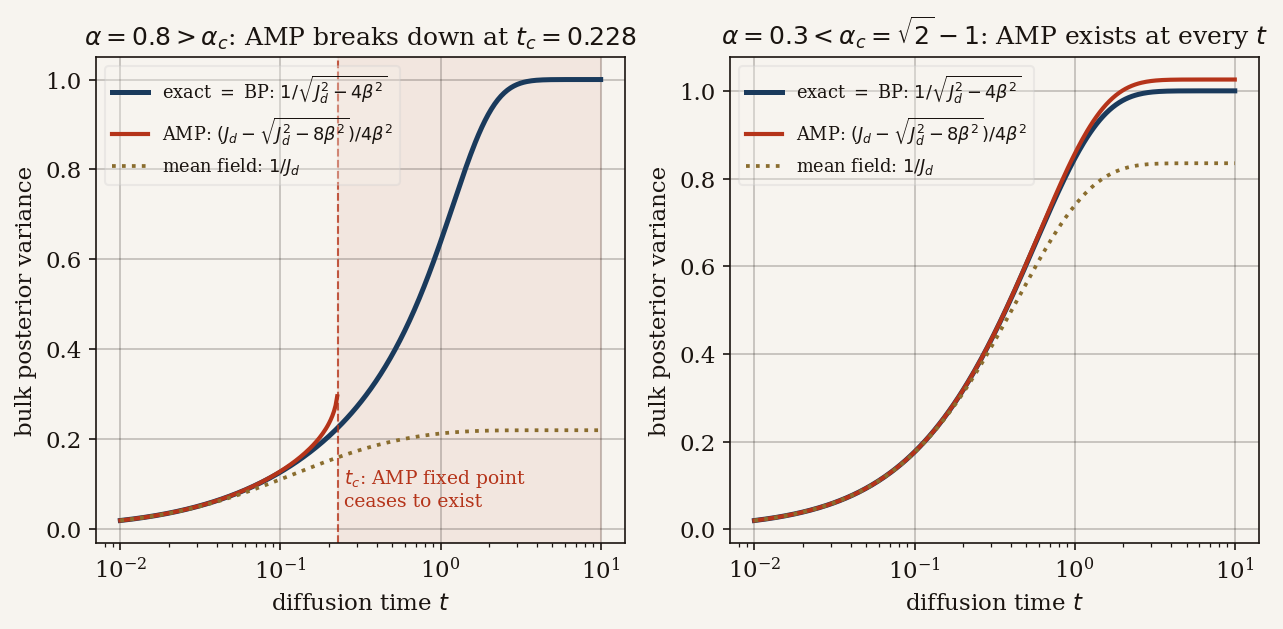
\includegraphics[width=\linewidth]{figures/fig_bulk_variance.png}
\caption{\textbf{The three closures in closed form.} Left
($\alpha = 0.8 > \alpha_c$): exact $=$ BP, AMP \eqref{eq:bp-amp-var}, and
mean field; the AMP branch terminates with a square-root singularity at
the exact breakdown time $t_c(0.8) = 0.228$ from \eqref{eq:bp-tc}
(shaded: no fixed point). Right ($\alpha = 0.3 < \alpha_c$): AMP exists at
every $t$ and slightly overestimates the variance, as predicted by
\eqref{eq:bp-weak}.}
\label{fig:bp-bulkvar}
\end{figure}

\begin{figure}[t]\centering
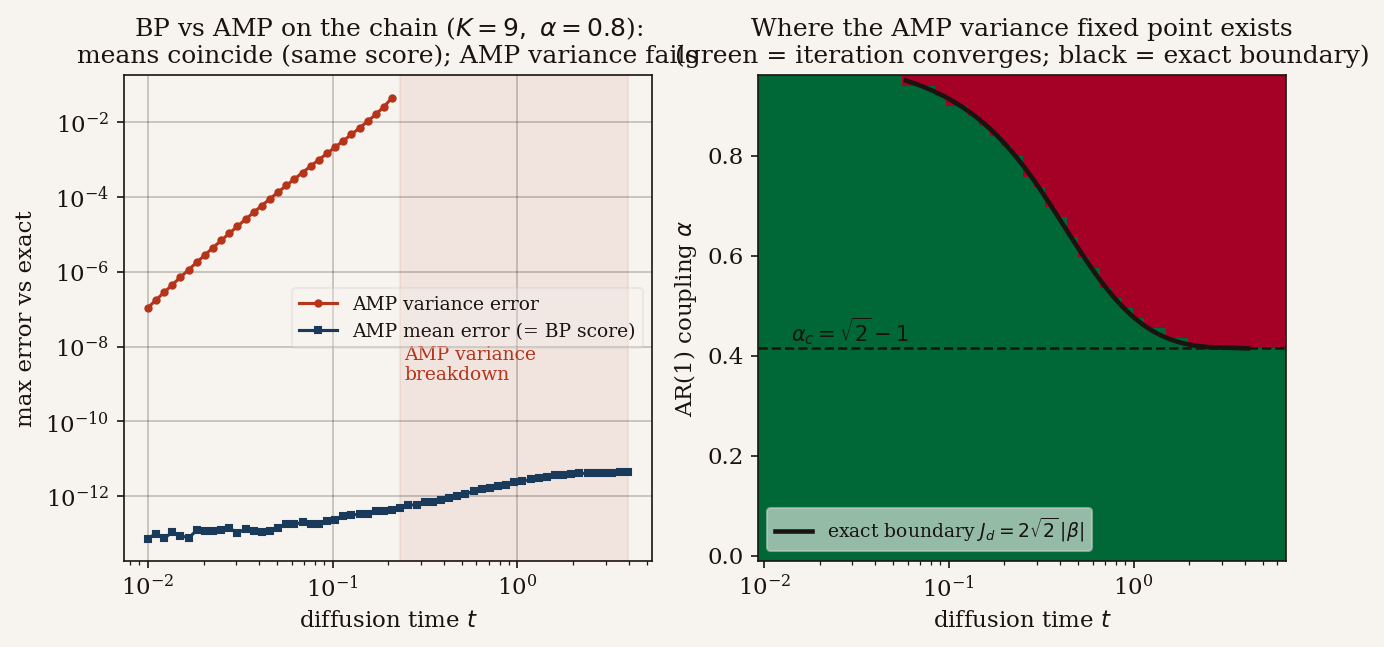
\includegraphics[width=\linewidth]{figures/fig_bp_vs_amp.png}
\caption{\textbf{BP vs AMP on a finite chain} ($K = 9$, $\alpha = 0.8$).
Left: the AMP \emph{mean} error ($\sim 10^{-12}$, flat in $t$: the score
is closure-independent, Theorem~\ref{thm:bp-same-score}) against the AMP
\emph{variance} error, which grows with $t$ until the closure stops
converging (shaded). Right: existence of the AMP variance fixed point in
the $(\alpha, t)$ plane; the black curve is the exact boundary
$t_c(\alpha)$ of \eqref{eq:bp-tc}, the dashed line
$\alpha_c = \sqrt{2}-1$; theory and iteration agree at all $180$ scanned
points.}
\label{fig:bp-vs-amp}
\end{figure}

Numerically, on a $K = 12$ chain at $\alpha = 0.8$: the AMP score error
stays at $10^{-13}$--$10^{-12}$ for every $t$, while the variance error is
$1.3 \times 10^{-4}$ at $t = 0.05$, $3.5 \times 10^{-2}$ at $t = 0.2$, and
past $t \approx 0.23$ the variance update has no positive fixed point at
all. The audit further verifies: the closed form \eqref{eq:bp-amp-var}
against the converged iteration to $2.5 \times 10^{-12}$; the existence
condition at all $180$ points of an $(\alpha, t)$ scan; $t_c$ against the
bisected flip point of the iteration to $6.6 \times 10^{-6}$ relative;
convergence below $\alpha_c$ even at $t = 50$; and the weak-coupling ratio
$(V_{\mathrm{AMP}} - V_{\mathrm{exact}})/(2\beta^4/J_d^5) \to 1$ within
$0.4\%$.

The supervision remark that framed this section --- the Gaussian message
assumption is a CLT statement, and ``a central limit theorem on two data
points is usually not right'' --- is thus made exact, with both halves
landing precisely where predicted. The \emph{conjecture} (Gaussian message
passing on the solved case recovers the known score) holds exactly: for BP
by algebraic closure, for AMP because the mean fixed point is
closure-independent. The \emph{objection} targets the variance closure,
and there it is not merely right but quantitative: a factor two in a
discriminant, a phase boundary \eqref{eq:bp-tc}, and a critical coupling
$\sqrt{2} - 1$. AMP is not wrong --- on a dense benchmark (random
$N = 600$ SPD precision) the same closure gets variances to
$1.7 \times 10^{-3}$ where mean field errs at $4 \times 10^{-2}$ --- it is
built for a different graph.

\section{The Gaussian closure beyond Gaussianity}\label{sec:bp-nongaussian}

On the Laplace chain of Chapter~\ref{ch:laplace}, BP is still exact in
principle but its messages are genuinely infinite-dimensional
(Remark~\ref{rmk:l-breakdown}). This is where the closure question becomes
a measurement. Two solvers are compared on identical data.

\paragraph{Exact reference: grid BP.} Messages are represented by their
values on $M$ equispaced points in $[-A, A]$ and updated by trapezoidal
quadrature --- option (iii) of Section~\ref{sec:bp-problem}. Calibration
on the exactly solvable Gaussian chain shows the trapezoid rule on
analytic, rapidly decaying integrands converges \emph{spectrally}
(aliasing error $\sim e^{-2\pi^2 \sigma^2/\dd x^2}$), so failure is
abrupt, not gradual: at $M = 101$, $A = 8$ the score error sits at the
$10^{-15}$ floor down to $t = 0.02$ and fails only when the likelihood
width $\sqrt{2t}$ approaches the grid step. The working configuration for
all non-Gaussian experiments is $M = 401$, $A = 8$ (reference $M = 801$),
with the resolution constraint $\sqrt{2t} \gtrsim 3\,\dd x$ checked
automatically; grid self-convergence error remains $10^4$--$10^7$ times
smaller than the effect being measured at every $t$. Within its validated
regime, grid BP \emph{is} the exact score.

\paragraph{The object under test: Gaussian-projected BP.} The same sweeps,
with every message forced into the Gaussian family by moment matching ---
the honest chain analogue of the AMP/TAP closure, and the algorithm one
would actually deploy when quadrature is unaffordable.

\paragraph{The error instrument.} All score errors are amplified
posterior-mean errors: for any two solvers producing means
$\widehat m, m_{\mathrm{ref}}$ and scores by Tweedie,
\begin{equation}
  \widehat s - s_{\mathrm{ref}}
  = \frac{e^{-t}}{\Deltat}\,
    \big( \widehat m - m_{\mathrm{ref}} \big),
  \qquad
  \frac{e^{-t}}{\Deltat} \sim \frac{1}{2t} \;\; (t \downarrow 0),
  \label{eq:bp-master-error}
\end{equation}
an exact identity (algebra, not approximation) whose numerical residual is
logged in every experiment and sits at $10^{-15}$--$10^{-12}$ throughout.
Equation \eqref{eq:bp-master-error} explains \emph{a priori} why small
diffusion times are the danger zone: whatever the closure does to the
posterior mean is amplified by $1/2t$ in the score.

\subsection{Findings on the Laplace chain}

On the Laplace chain ($\rho = 0.85$, $n = 40$, $60$ trials per $t$,
reference $M = 801$): the median relative score error of the Gaussian
closure is
\begin{center}
\begin{tabular}{@{}lcccc@{}}
\toprule
$t$ & $0.02$ & $0.08$ & $0.4$ & $2.4$ \\
\midrule
median relative score error & $0.39$ & $0.17$ & $3.5 \times 10^{-2}$
& $7.6 \times 10^{-5}$ \\
\bottomrule
\end{tabular}
\end{center}
with failure probability $\Prob(\mathrm{err} > 0.1)$ equal to $1$ for
$t \leq 0.08$ and $0$ for $t \geq 0.9$
(Figure~\ref{fig:bp-closure}). The closure error is thus of order tens of
percent in the small-$t$ regime and decays below $10^{-3}$ once diffusion
noise Gaussianises the tilted posteriors --- the quantitative form of the
supervision intuition that ``at long diffusion times the world is
Gaussian, so probably you have no problem''. Inspection of the worst
trials shows the mechanism: the reference belief is sharply non-Gaussian
(occasionally bimodal), the single Gaussian commits to a compromise mean,
and \eqref{eq:bp-master-error} amplifies the shift. The score
\emph{direction}, however, remains far more accurate than its magnitude
throughout: the median cosine similarity between projected and reference
scores is $0.92$ even at $t = 0.02$ (where the magnitude error is $39\%$),
exceeds $0.99$ for all $t \geq 0.12$, and the worst single trial of the
whole sweep stays above $0.78$.

\begin{figure}[t]\centering

\includegraphics[width=0.74\linewidth]{figures/nongaussian/laplace_closure_vs_grid_budget.png}
\caption{\textbf{Gaussian closure error on the Laplace chain} (median and
10--90\% band) against the grid error budget measured on identical data
($\rho = 0.85$): the closure error dominates the reference error by
$10^4$--$10^7$ at every $t$, so the measurement is trustworthy where it is
used.}
\label{fig:bp-closure}
\end{figure}

\subsection{Varying the innovation: what makes closure hard}

Sweeping six innovation families with \emph{identical} covariance
$\rho^{|i-j|}$ --- Laplace, Student-$t$ ($\nu = 5, 8$), and symmetric
Gaussian mixtures of increasing separation --- isolates the shape of the
innovation law as the only moving part. Three findings:
\begin{enumerate}
  \item \emph{Noise level dominates.} Every family's error decays to
  $\sim 10^{-3}$ or below by $t = 2.4$; all meaningful closure error lives
  at $t \lesssim 0.4$.
  \item \emph{Both signs of non-Gaussianity hurt; bimodality hurts most.}
  At $t = 0.05$, $\rho = 0.5$: strongly bimodal mixture $0.94$, Laplace
  $0.52$, Student-$t_{\nu=5}$ $0.32$, mildly bimodal mixture $0.07$. A
  single Gaussian cannot represent two posterior modes, and commits to the
  gap between them.
  \item \emph{Stronger correlation helps, not hurts.} Laplace at
  $t = 0.05$: error $0.43, 0.27, 0.13$ for $\rho = 0.5, 0.85, 0.95$.
  Informative neighbours act like extra Gaussian observations and
  Gaussianise the local tilted posterior; the naive intuition that message
  errors ``propagate farther'' at strong coupling is not what happens on
  chains.
\end{enumerate}

\subsection{Truncating the matrix versus truncating the inference}
\label{sec:bp-truncation}

The last supervision question --- take the exact score and truncate it to
tridiagonal: how bad? --- admits two inequivalent readings, and keeping
them apart turns out to matter. \emph{Truncate the answer} (variant a):
band the matrix, $\widehat S = -Q_t^{(b)} x$ with entries beyond
$|i - j| \leq b$ zeroed. \emph{Truncate the algorithm} (variant b): let
messages travel at most $r$ hops --- exact inference on the window
$x_{k-r}, \dots, x_{k+r}$, the local estimator of
Section~\ref{sec:g-locality}. Both estimators are linear in $x$, so their
RMS errors over the data law are deterministic traces --- no sampling.
At equal locality budget ($b = r = 1$, $K = 40$, $\alpha = 0.8$):
\begin{center}
\begin{tabular}{@{}lcccc@{}}
\toprule
relative RMS score error & $t = 0.05$ & $t = 0.3$ & $t = 1$ & $t = 3$ \\
\midrule
banded matrix ($b = 1$)      & $0.210$ & $0.302$ & $0.135$ & $0.0035$ \\
truncated inference ($r = 1$) & $0.123$ & $0.235$ & $0.130$ & $0.0035$ \\
\bottomrule
\end{tabular}
\end{center}
Two lessons. First, the cost of locality is non-monotone in $t$ and peaks
at intermediate times --- the same mid-diffusion window where the band of
$Q_t$ is fullest (Chapter~\ref{ch:gaussian}) and where generative
sampling spends its critical steps. Second, at small $t$ \emph{cutting the
algorithm beats cutting the answer} ($12.3\%$ vs $21.0\%$ at $t = 0.05$):
the windowed inference solves a correctly normalised problem on its
window, while zeroing entries of an inverse produces a matrix that is the
inverse of nothing and misstates the diagonal. The two coincide at large
$t$, where all off-diagonal content dies. The error of either truncation
decays geometrically in the allowed range, at the rate $q(\alpha, t)$ of
Theorem~\ref{thm:g-locality}.

\section{What this chapter established}\label{sec:bp-summary}

\emph{Exact} (proved, and verified to $10^{-12}$--$10^{-15}$): the factor
graph of the noisy chain is a tree; Convention-A BP computes its marginals
in $O(K)$; on the Gaussian chain all messages are Gaussian by algebraic
closure --- no CLT --- and BP $=$ Kalman smoother reproduces the matrix
score; the bulk BP fixed point \eqref{eq:bp-lambdastar} exists for all
$(\alpha, t)$; mean field, BP, and AMP share the exact score
(Theorem~\ref{thm:bp-same-score}); the AMP variance closure has the exact
phase boundary \eqref{eq:bp-tc}--\eqref{eq:bp-alphac} and the
weak-coupling law \eqref{eq:bp-weak}.
\emph{Numerical} (measured against validated exact references): the
Gaussian closure error on non-Gaussian chains ---
$\sim\!20$--$40\%$ at small $t$, $< 10^{-3}$ at large $t$, worst for
bimodal innovations, decreasing in $\rho$; and the locality comparison,
where truncated inference beats the truncated matrix at small $t$.
\emph{Heuristic}: the architecture reading --- local, convolution-like
score networks with receptive field sized by $q(\alpha, t)$ (or grown with
$t$) are near-optimal outside the mid-diffusion window, and the exactly
quantified penalty inside it is the price of locality, not an artefact.
These findings, their limitations, and the follow-up programme are
consolidated in the next chapter.
